\begin{table}
  \caption{Notation used in this article}
  \centering
  \begin{tabular}{l l l}
    \hline
    \multicolumn{1}{c}{Type of quantity} &\multicolumn{1}{c}{Symbol} & \multicolumn{1}{c}{Description} \\
    \hline
    Genetic parameters & $\psi$ & \multicolumn{1}{p{10cm}}{Mgf of the mutational effect size distribution }\\
                                         & $\frac{\theta}{2}$ & \multicolumn{1}{p{10cm}}{Per-locus mutation rate in units of coalescent time}\\
                                         & $m_i$ &  \multicolumn{1}{p{10cm}}{$i^{th}$ non-central moment of the mutational effect size distribution}\\
                                         & $\frac{\theta}{2}\mu_1$ & \multicolumn{1}{p{10cm}}{Rate that mutational bias shifts trait values in the infinitesimal limit}\\
                                         & $\frac{\theta}{2}\mu_2$ & \multicolumn{1}{p{10cm}}{Rate that variance accumulates in the infinitesimal limit}\\
                                         & $L$ & \multicolumn{1}{p{10cm}}{Number of potentially causal loci}\\
    Genealogy values &  $\Omega$ & \multicolumn{1}{p{10cm}}{Set of all possible branches in the genealogy of a given sample}\\
                                         & $\omega$ & \multicolumn{1}{p{10cm}}{A particular branch in a genealogy, defined by all individuals that branch subtends}\\
                                         & $\mathbf{T}$ & \multicolumn{1}{p{10cm}}{Random vector of branch lengths representing the entire genealogy at a locus}\\
                                         & $T_\omega$ & \multicolumn{1}{p{10cm}}{Length of branch $\omega$} \\
                                         & $T_{MRCA}$ & \multicolumn{1}{p{10cm}}{Time to the most recent common ancestor at a particular locus}\\
                                         & $\varphi_{\mathbf{T}}(\mathbf{s})$ & Mgf of the genealogy distribution \\
                                         & $\mathbf{s}$ & Vector of dummy variables for each possible branch\\
                                         & $s_\omega$ & Dummy variable for branch $\omega$ \\
                                         & $\mathbbm{T}_{k,n}$ & \multicolumn{1}{p{10cm}}{For a sample of exchangeable lineages, the amount of time that $k$ lineages remain in a sample of size $n$}\\
                                         & $\mathcal{T}_{a,b}$ & \multicolumn{1}{p{10cm}}{Pairwise coalescent time between a lineage sampled from $a$ and a lineage sampled from $b$, depending on the context, $a$ and $b$ may be either individuals or subpopulations}\\
                                         & $\tau_{a+b}$ & Sum of all branches ancestral to individuals $a$ and $b$\\
    Trait values & $\mathbf{Y}$ & Random vector of trait values \\
                                         & $Y_a$ & Trait value of individual $a$\\
                                         & $\varphi_{\mathbf{Y}}(\mathbf{k})$ & Mgf of the trait value distribution \\
                                         & $\mathbf{k}$ & \multicolumn{1}{p{10cm}}{Vector of dummy variables for each individual trait value}\\
                                         & $k_a$ & Dummy variable for individual $a$\\
                                         & $M_i$ & \multicolumn{1}{p{10cm}}{$i^{th}$ central moment of the trait value distribution in the entire population}\\
                                         & $CVV$ & \multicolumn{1}{p{10cm}}{Coefficient of variation of trait variance over evolutionary realizations of a population}\\
    \hline
  \end{tabular}
  \label{notation}
\end{table}

The model investigated here is of a trait controlled by $L$ unlinked potentially
causal loci and is shown schematically in Figure \ref{fig:schema}. Following
\citet{Kimura1969}, an infinite number of mutations are possible within each
locus (though the number of loci is finite) and rate that mutations affecting
the trait (causal mutations) arise is $\T$. That is, $\T$ is the rate for one
entire locus and not per nucleotide. An approximation restricting the number of
mutations per locus to at most one is considered in Section \ref{sec:lmr}.
Mutations receive values from a distribution of effect sizes. This distribution
is described by its moment generating function (mgf), $\psi$, and its
non-central moments, $m_i$. Individuals are haploid and their trait values are
determined by summing, both within and between loci, the effects of all
mutations occurring in that individual's history. Environmental effects are not
included. An extension to diploidy would be straightforward but is not
considered here.

Trait values are correlated between individuals because mutations fall on shared
portions of genealogies. The genealogy at a locus is represented by the random
vector of branch lengths, $\mathbf{T}$. An element $T_{\omega}$ of $\mathbf{T}$
is the branch length subtending only individuals in the set $\omega$. For
example, $T_{\{a,b\}}$ is the length of the branch ancestral only to individuals
$a$ and $b$. If such a branch does not exist for a given genealogy,
$T_{\{a,b\}}$ is set to zero. In this way $\mathbf{T}$ encodes both the branch
lengths and topology of a genealogy. $\Omega$ is the set of all possible
branches. For three sampled individuals, $a$, $b$, and $c$,
$\Omega=\{\{a\},\{b\},\{c\},\{a,b\},\{a,c\},\{b,c\}\}$ and
$\mathbf{T}=(T_{\{a\}},T_{\{b\}},T_{\{c\}},T_{\{a,b\}},T_{\{a,c\}},T_{\{b,c\}})$.
The distribution of genealogies is also described by its mgf,
$\varphi_{\mathbf{T}}$. Genealogies are independent between loci because of the
lack of linkage.

Phenotypic trait values are the random quantities we are interested in and will
hereafter be referred to simply as trait values. The vector of trait values in
the sampled individuals is $\mathbf{Y}$. If we had sampled individuals $a$, $b$,
and $c$, then $\mathbf{Y}=(Y_a,Y_b,Y_c)$. The contribution to the trait values
from a single locus is the change relative to the value in the most recent
common ancestor (MRCA) of the sample at that locus. $\mathbf{Y}$ is the sum over
contributions from $L$ loci, each measured with respect to an arbitrary
ancestral value. Since we do not know the ancestral value, we cannot directly
observe $\mathbf{Y}$. However, $\mathbf{Y}$ determines measurable quantities
such as differences in trait values between individuals as well as the sample
variance. The distribution of trait values is also studied through its mgf,
$\varphi_{\mathbf{Y}}$.

\begin{figure}
  \centering
  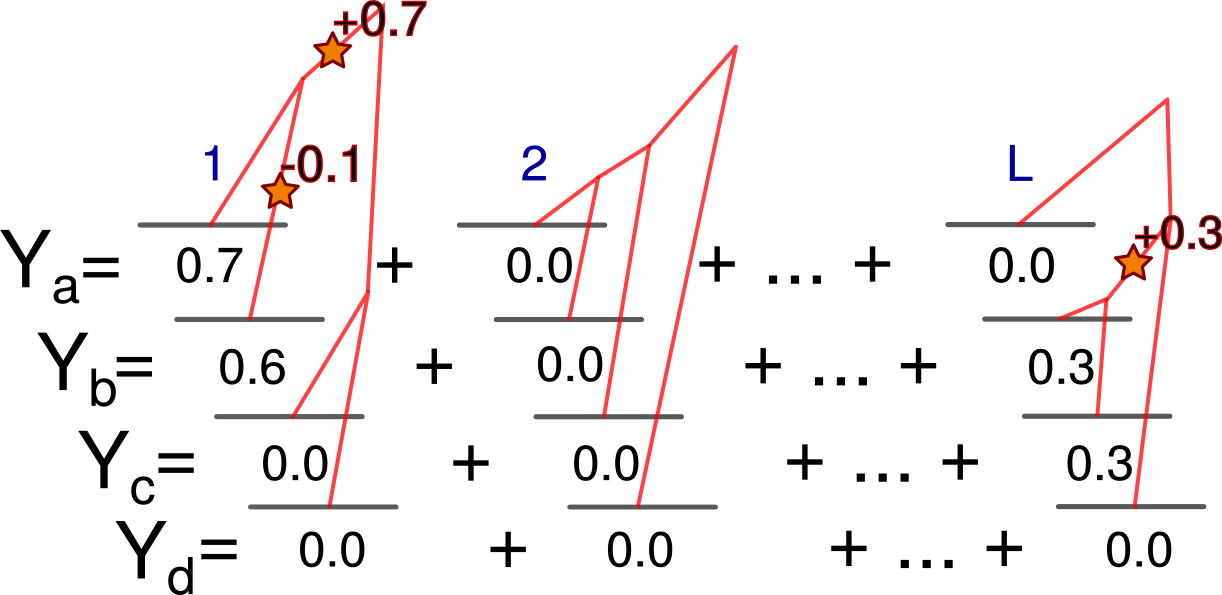
\includegraphics[width=0.9\textwidth]{./figures/schema.png}

  \caption{\textbf{A schematic representation of the model for how trait
  distributions arise from genealogical and mutational processes.} $L$ loci
  potentially affect the trait in a set of individuals and have independent
  genealogies. Mutations occur within loci as a Poisson process and act
  additively to give individual trait values. Many loci with the potential to
  affect the trait may receive no mutations.}

  \label{fig:schema}
\end{figure}

We call those quantities not influenced by the genealogical process ($L$, $\T$,
$\psi$) the genetic parameters of the trait. Another quantity useful for
describing a trait's distribution is its sparsity. Sparsity should reflect how
many mutations segregating in the population influence the trait, with a more
`sparse' trait being one affected by fewer segregating mutations. Formally, we
measure sparsity as the average number of pairwise differences between two
randomly chosen haplotypes at loci affecting the trait. A trait with fewer
causal pairwise differences is more sparse. Sparsity thus depends both on the
genetic parameters through the mutation rate and the number of potentially
causal loci, and on demography through the distribution of coalescence times.

In populations of exchangeable individuals, a useful way to summarize the
distribution of genealogies is through the moments of $\mathbbm{T}_{k,n}$ which
denotes the amount of time that $k$ lineages remain in the genealogy of a sample
of size $n$. The pairwise coalescent time between a lineage in individual $a$
and in individual $b$ is written as $\mathcal{T}_{a,b}$. When considering
structured populations, $\mathcal{T}_{a,b}$ is also used to denote the
coalescence time between a randomly chosen lineage from subpopulation $a$ and a
randomly chosen lineage from subpopulation $b$. Table \ref{notation} provides a
reference for the notation used in this article. 

% A final set of quantities are defined for sums of branch lengths. Let
% $\tau_{a+b}$ be the sum of all branches ancestral to both $a$ and $b$, and
% $\tau_{a/b}$ be the sum of all branches ancestral to $a$ but not $b$. Extensions
% of this for more than two individuals are also used. The same notation is used
% when referring to sets of branch indices. So $\Omega_{a+b}$ and $\Omega_{a/b}$
% would be the sets of branches added to get $\tau_{a+b}$ and $\tau_{a/b}$
% respectively.

%%% Local Variables:
%%% TeX-master: "short_report.tex"
%%% End:
